\documentclass[12pt]{article}

\usepackage{fullpage}
\usepackage[utf8]{inputenc}
\usepackage[T1]{fontenc}
\usepackage{indentfirst}
\usepackage{graphicx}
\usepackage{booktabs}
\graphicspath{ {images/} }
\usepackage[portuguese]{babel}

\begin{document}
\begin{titlepage}
    
\includegraphics[width=0.3\textwidth]{fctUnlLogo.jpg}
    \begin{center}
        \vspace{0.5cm}

        \begin{Large}
        	\underline{\textbf{Opção A}}\\
        \end{Large}
        
        \textbf{\emph{\emph{Publish-Subscribe} utilizando redes estruturadas}}
               
        \vspace{0.3cm}

		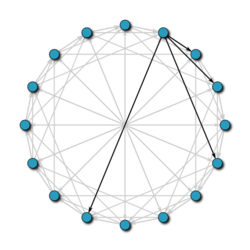
\includegraphics[width=0.4\textwidth]{Chord_network.png}
		
        \vspace{0.3cm}
        
        Trabalho realizado por:
        
        \vspace{0.5cm}

		\begin{table}[htbp]
		\centering
        	\begin{tabular}{c c}
				\textbf{Luís Duarte Oliveira, nº 41894} & \textbf{Daniel Pimenta, nº 45404}\\
				\texttt{ld.oliveira@campus.fct.unl.pt} & \texttt{d.pimenta@campus.fct.unl.pt}\\
			\end{tabular}
		\end{table}
		
		\begin{table}[htbp]
		\centering
        	\begin{tabular}{c}
				\textbf{Luís Martins, nº 45640}\\
				\texttt{lg.martins@campus.fct.unl.pt}\\
			\end{tabular}
		\end{table}
		
        \vspace{0.5cm}
        
        Para a cadeira de:
        
        Algoritmos e Sistemas Distribuídos (ASD)
        
        \vspace{0.5cm}

		Professor regente: 
		João Leitão
		
		Professor responsável:
		Nuno Preguiça
		
        \vspace{0.5cm}
                
        Departamento de Informática\\
        Faculdade de Ciências e Tecnologia\\
        Universidade Nova de Lisboa\\
        17 de novembro de 2018
    \end{center}
\end{titlepage}

\newpage
\tableofcontents

\newpage
\listoffigures

\newpage
\listoftables

\newpage
\section{Introdução}

No âmbito da cadeira de Algoritmos e Sistemas Distribuídos, foi-os proposto o projeto, de implementar um sistema de \emph{Publish-Subscribe}, em cima de uma \emph{distributed hash table} (DHT).

DHT é um modelo de rede estruturada, com capacidade para guardar dados de forma distribuída, em cada nó da mesma.

Na implementação deste sistema, constatamos a complexidade desta classe de algoritmos. Ao realizar testes sobre uma rede deste tipo, aprendemos a identificar as propriedades do sistema.

\newpage
\section{Visão global}

Este sistema pode ser decomposto em 3 camadas. 

A primeira, é a camada que dá suporte ao sistema. Esta, no nosso caso corresponde a implementação do algoritmo Chord \cite{b2}. 

A segunda, é a camada relacionada com o sistema de \emph{Publish-Subscribe}. Esta, é responsável pela criação e subscrição dos respetivos tópicos de interesse, a cada individuo na rede. Com estas subscrições, será possível a troca de mensagens dentro de cada tópico. 

A terceira e última, é a camada de teste. Esta, é responsável pela recolha e processamento dos dados de teste para futura análise.

As primeiras duas camadas, foram implementadas tendo como guia os materiais da cadeira de ASD \cite{b1}.

A implementação deste sistema, foi feito com a linguagem computacional de Scala \cite{b3}, utilizando o conjunto de ferramentas do Akka \cite{b4}.

\newpage
\section{Visão global detalhada}

Nesta secção, iremos explicar por escrito, em pormenor, os detalhes de cada uma das camadas anteriormente mencionadas.

\newpage
\subsection{Chord}

O Chord quando arranca, define o predecessor do nó a nulo e o sucessor do nó, como ele mesmo. No caso de não ser o primeiro, inicializa o predecessor a nulo e o sucessor com o resultado da função com o objetivo de encontrar o sucessor.

A função de encontrar o sucessor, funciona com a seguinte condição, "determinado nó, pede ajuda ao nó anterior, para encontrar o nó posterior".

As restantes funções do algoritmo, têm como objetivo manter o sistema num estado estável e correto. Estas, são chamadas regularmente, do início ao fim da execução.

A função de estabilização, verifica se o nó contém o sucessor correto e notifica o sucessor, sobre quem é o seu predecessor.

A função de arranjar os \emph{fingers}. É importante verificar se os \emph{fingers} estão a apontar para os valores corretos, caso contrário torna a execução do algoritmo impossível. Esta função, analisa gradualmente, \emph{finger} a \emph{finger}, se cada \emph{finger} de cada nó tem os valores certos. 

Por último, temos a função de verifica se o predecessor é um nó ativo, ou não.

\newpage
\subsection{Publish-Subscribe}

O \emph{Publish-Subscribe} tem como função, permitir os clientes fazerem a subscrição em determinados tópicos e submeterem mensagens nos mesmos.

Cada cliente pode publicar mensagens em cada tópico, sendo as mesmas disseminadas por todos os subscritores. As mensagens são publicadas, utilizando o comando \emph{route}.

Regularmente os clientes verificam se os tópicos, ainda estão ativos. Caso não estejam, então é criado um novo tópico.

Periodicamente, os nós que têm tópicos, verificam se o tópico é procurado. Caso não seja, o tópico é apagado.

\newpage
\subsection{Aplicação de teste}

TO DO...

\newpage
\section{Pseudo-código e arquitetura}

TO DO...

\newpage
\subsection{Chord}

O pseudo-código do Chord, segue rigorosamente o algoritmo apresentado pelo professor, nos slides da cadeira de ASD \cite{b1}.

\begin{figure}[htbp]
	\centering
	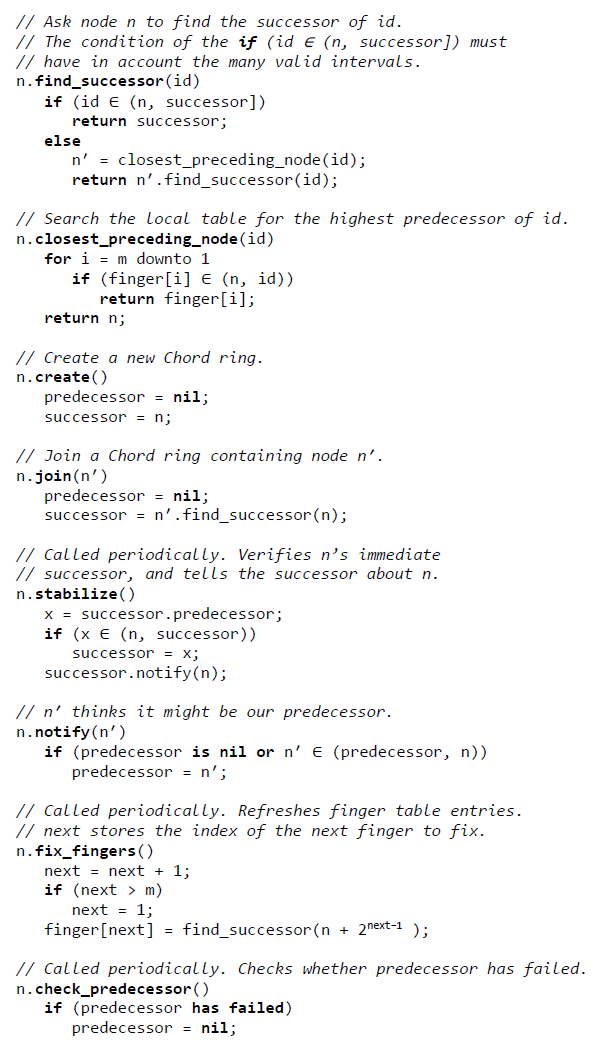
\includegraphics[height=0.96\textwidth]{pseudoChord.png}
	\caption{Pseudo-código do algoritmo Chord.}
	\label{fig:chord}
\end{figure}

\newpage
\subsection{Publish-Subscribe}

TO DO...

\newpage
\subsection{Aplicação de teste}

TO DO...

\newpage
\section{Avaliação dos resultados}

TO DO...

\subsection{Experiências}

TO DO...

\subsection{Resultados com observações}

TO DO...

\newpage
\section{Conclusão}

TO DO...

\newpage
\begin{thebibliography}{00}
\bibitem{b1} Leitão, J. (2018). Materiais da cadeira de ASD. FCT/UNL.
\bibitem{b2} Stoica, I., Morris, R., Liben-Nowell, D., Karger, D. R., Kaashoek, M. F., Dabek, F., \& Balakrishnan, H. (2003). Chord: A scalable peer-to-peer lookup protocol for Internet applications. IEEE/ACM Transactions on Networking, 11(1), 17–32. https://doi.org/10.1109/TNET.2002.808407
\bibitem{b3} Fédérale, É. P., \& (EPFL), L. (n.d.). Scala. Retrieved November 17, 2018, from https://www.scala-lang.org/
\bibitem{b4} Lightbend, I. (n.d.). Akka. Retrieved November 17, 2018, from https://akka.io/
\bibitem{b5} Penman, T. (n.d.). Implementing a Distributed Hash Table with Scala and Akka. Retrieved November 17, 2018, from http://tristanpenman.com/blog/posts/2015/11/26/implementing-a-dht-with-scala-and-akka/
\end{thebibliography}

\end{document}